\documentclass[11pt,a4paper]{article}
%\usepackage{eulervm}
%\usepackage{charter}
\usepackage[utf8]{inputenc}
\usepackage{amsmath,amssymb}
\usepackage{mathrsfs} 
\usepackage{fancyhdr}
\usepackage{enumerate}
\usepackage{tikz,tkz-tab}
%\usepackage{tkz-euclide}
\usepackage{tikz-3dplot}
\usetikzlibrary{arrows,calc,intersections,angles,patterns,shapes.geometric}
\usepackage[most]{tcolorbox}
\usepackage{pgfplots}
\usepgfplotslibrary{fillbetween}
\pgfplotsset{compat=1.9}

\usepackage[top=1cm, bottom=1.5cm, left=1.5cm, right=1.5cm] {geometry}
\usepackage[hidelinks,unicode]{hyperref} %\usepackage[unicode, bookmarks=false]{hyperref}
\usepackage{currfile}
%\usepackage[loigiai]{ex_test} 
%   \renewcommand{\FalseEX}{\stepcounter{dapan}\textbf{\color{blue}\Alph{dapan}.}}
\usepackage[solcolor]{ex_test} 
    \renewcommand{\TrueEX}{\stepcounter{dapan}{\circled{\textbf{\Alph{dapan}}}}}

\newcommand{\solutionhide}[1]{%
\def\True{\setcounter{numTrue}{\thedapan}\setcounter{numTrueSol}{\thedapan}}
    \AtBeginEnvironment{#1}{%
        \renewcommand{\loigiai}[1]{%
}}}
\newtcolorbox[auto counter]{boxEx}{
    breakable,top=2.2mm,fonttitle=\bfseries,title={
        \textbf{exercice} \thetcbcounter:},enhanced,before skip=0mm,after skip=5mm,boxsep=-1mm,boxrule=1pt,colframe=cyan,colback=cyan!5,sharp corners,rounded corners=southeast,arc=3mm,drop fuzzy shadow=cyan!50!gray,coltitle=blue,attach boxed title to top left={xshift=0mm,yshift=-\tcboxedtitleheight},boxed title style={interior empty,frame code={
            \fill([xshift=-2mm]frame.north east)arc(180:0:1mm);
            \fill[right color=cyan,left color=yellow,middle color=green!50] ([shift={(.3,.1)}]frame.north west)--([shift={(-.1,.1)}]frame.north east)[rounded corners=1mm]--([xshift=-2mm]frame.north east)--([xshift=-3mm]frame.south east)--([xshift=1mm]frame.south west)--([xshift=2mm]frame.north west)--cycle;
}}}
%--------------------------------------------------------
\newtcolorbox[auto counter]{exo}{
    breakable,top=2.2mm,fonttitle=\bfseries,title={
        \textbf{Exercice} \thetcbcounter:},enhanced,before skip=5mm,after skip=5mm, boxsep=-1mm,boxrule=1pt,colframe=cyan,colback=cyan!5,sharp corners,rounded corners=southeast,arc=3mm,
       % drop fuzzy shadow=cyan!50!gray,
        coltitle=blue,attach boxed title to top left={xshift=0mm,yshift=-\tcboxedtitleheight},boxed title style={interior empty,frame code={
            \fill([xshift=-2mm]frame.north east)arc(180:0:1mm);
            \fill[right color=gray,left color=gray!50,middle color=gray!50] ([shift={(.3,.1)}]frame.north west)--([shift={(-.1,.1)}]frame.north east)[rounded corners=1mm]--([xshift=-2mm]frame.north east)--([xshift=-3mm]frame.south east)--([xshift=1mm]frame.south west)--([xshift=2mm]frame.north west)--cycle;
}}}
%---------------------------------------------------------
\def\beginbox{\begin{boxEx}}
\def\endbox{\end{boxEx}}
\newcommand{\solutionshow}[1]{%
\def\loigiaiEX{\centerline{\color{teal}Loi}}
    \AtBeginEnvironment{#1}{%
        \beginbox
        \renewcommand{\loigiai}[1]{%
        \endbox
        \noindent
        \begin{onlysolution}{\color{brown}##1}
        \end{onlysolution}
}}}

\def\colorEX{}%
\renewtheorem{ex}{\color{red}\textbf{ex}}
\newcommand\gbox[1]{\noindent
\begin{tikzpicture}[gray,ultra thin]
\def\gw{1.77} \def\gh{.67}\def\gl{.3}\def\gt{.05}
\path(0,0)node[rectangle,draw=white,fill=white,inner sep=4pt] (box){\begin{minipage}{\textwidth}{#1}\end{minipage}};
\foreach\i in{0,...,10}\draw([shift={(\i*\gw+\gl,\gt)}]box.north west)--([shift={(\i*\gw+\gl,\gt-5*\gh)}]box.north west);
\foreach\i in{0,...,5}\draw([shift={(\gl,\gt-\i*\gh)}]box.north west)--([shift={(10*\gw+\gl,\gt-\i*\gh)}]box.north west);
\end{tikzpicture}
}
\newcommand{\boxanss}{
	\renewenvironment{Solution}[1]
	{\begin{minipage}{0.09\linewidth}\hfill{\color{blue}##1~-~}\color{purple}}{\end{minipage}}
}
\everymath{\displaystyle}
\usepackage{esvect}
\def\madethi{ma die sol: 000}
\def\vec{\overrightarrow}
\newcommand{\hoac}[1]{ 
	\left[\begin{aligned}#1\end{aligned}\right.}
\newcommand{\heva}[1]{
	\left\{\begin{aligned}#1\end{aligned}\right.}
\renewcommand{\baselinestretch}{1.4}
\usepackage{fancyhdr}
\pagestyle{fancy}
\fancyhf{}
\renewcommand{\headrulewidth}{0pt}
\lfoot{\scriptsize Anne scolaire 2022}
\rfoot{\scriptsize Trang \thepage/1\, --- \madethi }
\begin{document}
%%\centerline{\textbf{CÂU HỎI TRẮC NGHIỆM}}
%%\vspace{1em}
%%\solutionhide{ex}
%%\Opensolutionfile{ans}[ansde]
%%\setcounter{ex}{0}
\begin{ex}%[Cau 1]
$A$  $B$  $f(x)=x^3-3x^2+m$ $m\neq0$.  $m$  $OAB$  $3x+3y-8=0$.
\choice
{\True $m=5$}
{$m=2$}
{$m=6$}
{$m=4$}
\loigiai{
{\bf bgf 1}

   $f'(x)=3x^2-6x=0\iff\hoac{x=0&\implies y=2\\ x=2&\implies y=m-4}\implies A(0;2),~B(2;m-4)$
 
  $G$  $\triangle OAB$,  $G\left(\frac23;\frac{2(m-2)}3\right)$
 
 $G$  $3x+3y-8=0\iff 2+2(m-2)-8=0\iff m=5$
 \\ {\bf ex 2}

  $M(x_o;y_o)$  $AB$. 
 
  $f''(x_o)=0\iff 6x_o-6=0\iff x_o=1\implies y_o=m-2\implies M(1;m-2)$
 
  $G$  $\triangle OAB$,  $\vec{OG}=\frac23\vec{OM}=\left(\frac23;\frac{2(m-2)}3\right)$
 
 $G$  $3x+3y-8=0\iff 2+2(m-2)-8=0\iff m=5$
}

\end{ex}

\begin{ex}%[Cau 2]
 $y=f(x)$ 
\immini{ bla bla ...
\choice[2]
{$(1; 3)$}
{$(3; 1)$}
{\True $(-1; -1)$}
{$(1; -1)$}
}{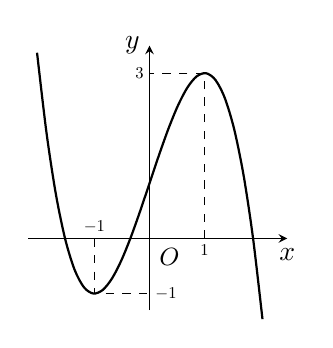
\begin{tikzpicture}[scale=.7]
\draw[-stealth] (-2.2,0) -- (2.5,0) node[below]{$x$};
\draw[-stealth] (0,-1.3) -- (0,3.5) node[left]{$y$};
\draw (0,0) node[below right]{\small $O$};
\draw[dashed] (-1,0)|-(0,-1)(1,0)|-(0,3);
\draw[thick,smooth] plot[domain=-2.04:2.05](\x,{-(\x)^3+3*(\x)+1});
\path(1,0)node[below,scale=.6]{$1$} (-1,0)node[above,scale=.6]{$-1$}
(0,-1)node[right,scale=.6]{$-1$} (0,3)node[left,scale=.6]{$3$};
\end{tikzpicture}}
\loigiai{
bla bla lbla ldl ....... $(-1;-1)$
}
\end{ex}

%%\Closesolutionfile{ans}
%%\centerline{\bf ------------ HẾT ------------}
%%\newpage
%%\setcounter{page}{1}
\lfoot{\scriptsize bla lld llsd}
\rfoot{\scriptsize Trang \thepage/1\, --- \madethi }
%%\centerline{\textbf{BẢNG KHOÁ CÂU TRẮC NGHIỆM}}
%%\gbox{\boxanss\begin{flushleft}{\bf\input{ansde}}\end{flushleft}}
\centerline{\textbf{de la de la }}
\vspace{-1cm}
\solutionshow{ex}
\Opensolutionfile{ans}[ansda]
%\setcounter{ex}{0}
\begin{ex}%[Cau 1]
$A$  $B$  $f(x)=x^3-3x^2+m$ $m\neq0$.  $m$  $OAB$  $3x+3y-8=0$.
\choice
{\True $m=5$}
{$m=2$}
{$m=6$}
{$m=4$}
\loigiai{
{\bf bgf 1}

   $f'(x)=3x^2-6x=0\iff\hoac{x=0&\implies y=2\\ x=2&\implies y=m-4}\implies A(0;2),~B(2;m-4)$
 
  $G$  $\triangle OAB$,  $G\left(\frac23;\frac{2(m-2)}3\right)$
 
 $G$  $3x+3y-8=0\iff 2+2(m-2)-8=0\iff m=5$
 \\ {\bf ex 2}

  $M(x_o;y_o)$  $AB$. 
 
  $f''(x_o)=0\iff 6x_o-6=0\iff x_o=1\implies y_o=m-2\implies M(1;m-2)$
 
  $G$  $\triangle OAB$,  $\vec{OG}=\frac23\vec{OM}=\left(\frac23;\frac{2(m-2)}3\right)$
 
 $G$  $3x+3y-8=0\iff 2+2(m-2)-8=0\iff m=5$
}

\end{ex}

\begin{ex}%[Cau 2]
 $y=f(x)$ 
\immini{ bla bla ...
\choice[2]
{$(1; 3)$}
{$(3; 1)$}
{\True $(-1; -1)$}
{$(1; -1)$}
}{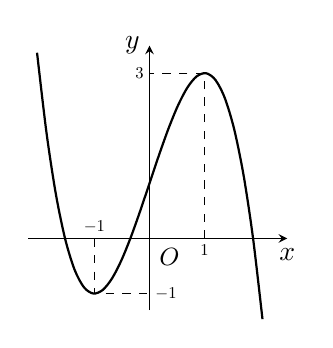
\begin{tikzpicture}[scale=.7]
\draw[-stealth] (-2.2,0) -- (2.5,0) node[below]{$x$};
\draw[-stealth] (0,-1.3) -- (0,3.5) node[left]{$y$};
\draw (0,0) node[below right]{\small $O$};
\draw[dashed] (-1,0)|-(0,-1)(1,0)|-(0,3);
\draw[thick,smooth] plot[domain=-2.04:2.05](\x,{-(\x)^3+3*(\x)+1});
\path(1,0)node[below,scale=.6]{$1$} (-1,0)node[above,scale=.6]{$-1$}
(0,-1)node[right,scale=.6]{$-1$} (0,3)node[left,scale=.6]{$3$};
\end{tikzpicture}}
\loigiai{
bla bla lbla ldl ....... $(-1;-1)$
}
\end{ex}

\Closesolutionfile{ans}
\begin{exo}
\hspace{2.5cm}yahya
\vspace{2cm}
\end{exo}
\end{document}
